\chapter{微译器设计与实现}\label{chap:MUT}

上文\ref{sec:bt_overhead_all}我们通过分析发现二进制翻译器的主要开销来源于指令集语义差异和间接跳转开销。

指令集语义差异的一种常见的解决办法是在宿主指令集中添加指令集扩展,来接近客户指令集的语义,例如LoongArch指令中添加的LBT二进制翻译扩展指令。
但这样会增加宿主指令集的复杂度,更加剧了指令集的历史包袱,同时添加指令集扩展也难以支持多种指令集的兼容。
我们从X86处理器定义的微码指令集中得到启发,微码是一种内部指令集,不对外暴露给用户和编译器,并且可以随着处理器的演进而不断迭代优化,不需要考虑历史兼容包袱。

我们希望能否定义一套融合微码,作为一种内部指令集,包含各个指令集的并集,对外不暴露给用户,而是通过二进制翻译器将客户指令翻译为融合微码指令,从而实现多指令集的兼容。
在这个层面上,二进制翻译器类似于一个软件译码器,将客户指令翻译为融合微码指令,而CPU则类似于一个虚拟机,执行融合微码指令。
我们不太方便直接做一个硬件译码器,对外直接支持X86和RISCV等多个指令集,因为这样可能会有授权问题。

而对于间接跳转开销,X86的微码缓存天然的就能解决这个问题,因为硬件上的微码缓存维护好了X86指令地址和微码指令地址的映射关系,可以通过简单的线性映射关系访问的微码指令地址,
而不需要软件上复杂的哈希表查询逻辑,这样可以大大减少间接跳转的开销。
% 一条X86指令译码为多条微码指令,这个和一条宿主指令翻译为多条客户指令类似,都是一种一对多的关系。

为此我们借鉴X86微码和微码缓存的概念,提出了一种多架构软硬协同的二进制翻译技术——\textbf{微译器},
通过\textbf{融合微码}缩小了指令集语义差异,
通过\textbf{翻译缓存}来消除间接跳转开销,提高了二进制翻译器的性能。

\section{微译器整体架构}

\begin{figure}[h]
  \centering
  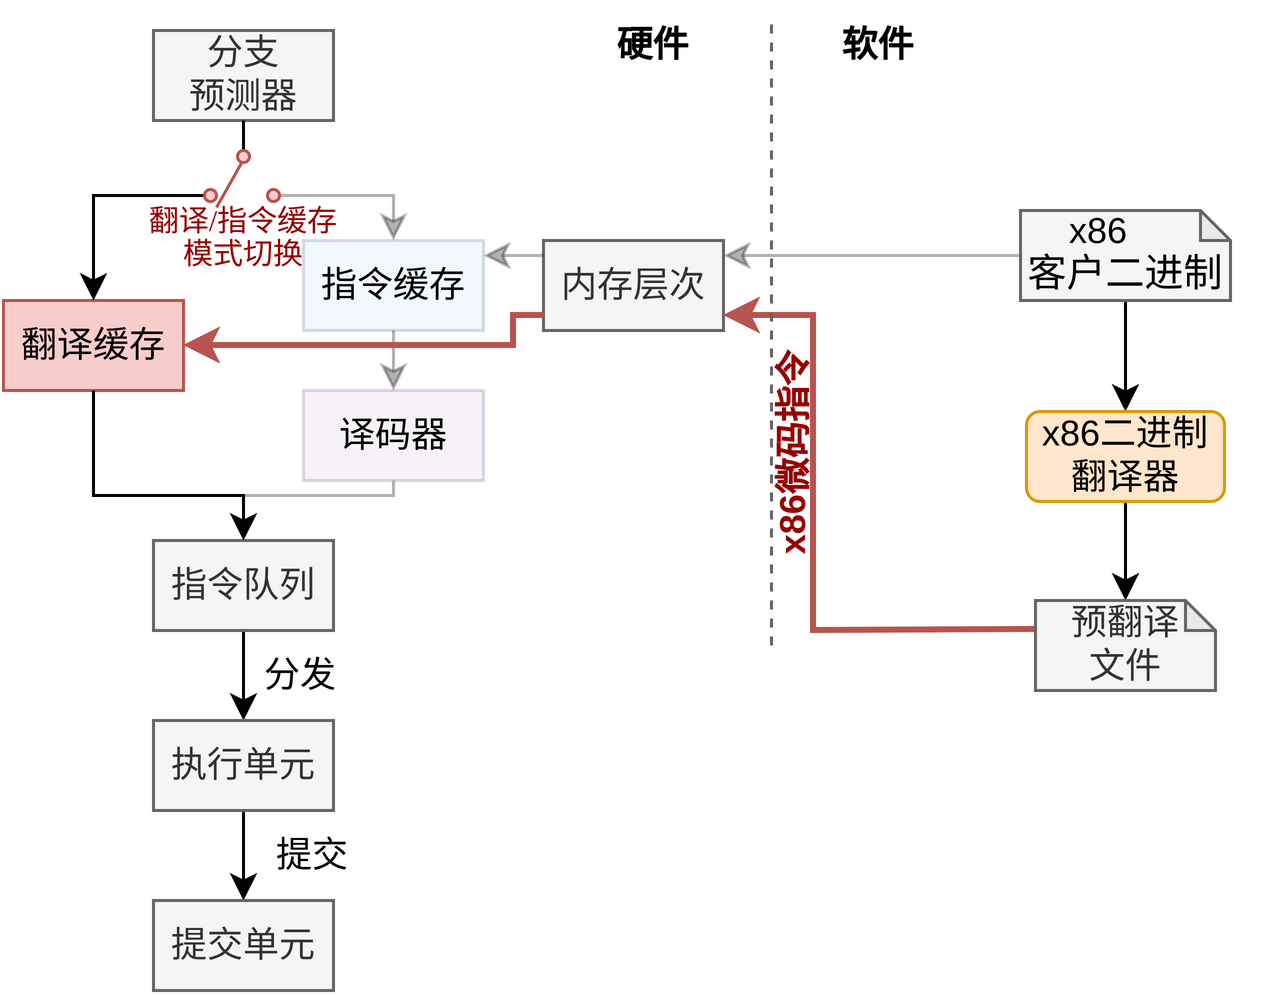
\includegraphics[width=1\linewidth]{./image/front_end_transutor.pdf}
  \caption{微译器整体架构图}
  \label{img:front_end_transutor}
\end{figure}

如图\ref{img:front_end_transutor}展示了微译器的整体架构。

% \subsection{硬件部分}

在硬件部分,引入了\textbf{翻译缓存}(Translation Cache),该缓存作为一级缓存负责存储预翻译的微码指令集,替代了原本的微码缓存。
翻译缓存的每行组织形式和微码缓存类似,都是前面部分存放微码指令(这里为融合微码指令,下一节详细介绍),
后面存放立即数,微码指令和立即数相向生长,中间可能有空洞,产生新的开销,后文会提出对应的优化方案。

此外与传统微码架构不同,微码缓存数据是直接来源于CPU和指令缓存,通过硬件译码器进行译码并存入微码缓存中;
而翻译缓存通过软件的二进制翻译“译码”,透过内存层次(从内存加载到L3 Cache, 再到L2Cache, 最后到微码缓存)进行填充,
取代了传统的指令缓存和译码器的角色。
在传统X86架构下,取指部件会同时查询指令缓存和微码缓存;
而在微译器架构下,取指部件仅查询翻译缓存,硬件的译码器被软件的二进制翻译器取代。
为了兼容传统的X86处理器模式,我们添加了一个模式切换逻辑,可以切换回使用硬件译码器进行译码,这样可以在不改变原有X86处理器的基础上实现微译器的功能。

% \subsection{软件部分}

在软件部分,引入了静态和动态二进制翻译器。
程序首先通过静态二进制翻译器被翻译成融合微码指令,并被写入预翻译文件,存储在硬盘中。
在客户程序执行阶段,预翻译文件被加载到内存中,程序计数器被设置为客户程序的入口。
取指部件从翻译缓存中取指,若翻译缓存或内存层次命中,则从翻译缓存取指,发送到处理器后端执行,不断取指执行。
若翻译缓存和内存层次均未命中(例如存在自修改代码等),说明客户指令还未翻译,此时会调用动态二进制翻译器进行实时翻译,
并将翻译结果写入翻译缓存,再取指执行。

\section{二进制翻译器}

\section{翻译缓存}

\section{融合指令集}
本节详细介绍重要的一个概念——融合微码。“融合”代表它能融合了多种指令集的特征,
包括X86和RISCV,未来还可以支持ARM,MIPS等其他指令集,
或许叫统一微码也更好理解。但融合并非简单的把所有指令集简单拼接就好,这会造成指令集冗余,挤占有限的编码空间。

“微码”这个名字主要由于它在翻译缓存中的组织形式和传统的X86微码缓存组织形式类似,并且更像是不同指令集的更低级表现形式;
此外目前第一代的融合微码是在原有的Gem5 X86微码上扩充的,
所以便于理解仍然保留融合微码的名字。

但事实上,融合微码有很大特征很像一个“RISC指令集”。
由于我们的融合微码指令是需要存储在磁盘中的,并不像传统X86微码只是作为一个“暂时指令”存在于CPU运行期间,
所以融合微码指令需要像普通指令集一样进行\textbf{编码},
编译器(或者二进制翻译器)把指令\textbf{编码}为定长的融合微码指令,并存储于磁盘中。
CPU再从磁盘中加载融合微码指令,\textbf{解码}为CPU识别的信息,这一阶段也叫“译码阶段”。
因此从这个角度来说,加上指令定长、只能操作寄存器、指令间关系被简化等特征,融合微码很像一个普通的“RISC指令集”。
因此融合微码类似传统指令集概念,也是有编码空间的概念。